\documentclass[11pt, oneside]{article}   	% use "amsart" instead of "article" for AMSLaTeX format
\usepackage{geometry}                		% See geometry.pdf to learn the layout options. There are lots.
\geometry{letterpaper}                   		% ... or a4paper or a5paper or ... 

\usepackage[english]{babel}
\usepackage{url, verse}
\usepackage{pstricks, tikz}
\usepackage[T1]{fontenc}
\usepackage{setspace}
\usepackage{graphicx, wrapfig, capt-of}
\usepackage[normalem]{ulem} %for \sout
\usepackage{amssymb}
\usepackage{color}
\usepackage{tipa}
\usepackage{multicol}

\usepackage{stackengine}
\usepackage{array}
\newcolumntype{P}[1]{>{\centering\arraybackslash}p{#1}}
\newcolumntype{M}[1]{>{\centering\arraybackslash}m{#1}}
\usepackage{hhline,multirow}
\newcommand*\rot{\rotatebox{90}}

\usepackage{linguex} %declare this package after tipa and graphicx
\renewcommand{\firstrefdash}{}
\usepackage{qtree}
\usepackage{tree-dvips} %copy tree-dvips folder to make this work
\qtreecenterfalse

\usepackage{fancyhdr}
\pagestyle{fancy}{
\fancyhead[L]{Roberto Petrosino}
\fancyhead[C]{LING2010Q}
\fancyhead[R]{2: Phonetics}
\renewcommand{\footrulewidth}{0pt}
\renewcommand{\headrulewidth}{0pt}}

\newenvironment{packed_enum}{
\begin{enumerate}
  \setlength{\itemsep}{1pt}
  \setlength{\parskip}{0pt}
  \setlength{\parsep}{0pt}
}{\end{enumerate}}

\newenvironment{packed_item}{
\begin{itemize}
  \setlength{\itemsep}{1pt}
  \setlength{\parskip}{0pt}
  \setlength{\parsep}{0pt}
}{\end{itemize}}

\renewcommand{\labelitemiii}{$\diamond$}


\title{{\normalsize LING 2010Q -- {\scshape Fall 2017}} \\ {\bfseries 2 - Phonetics}, or: \\ {\itshape the science of sounds -- level of abstractness: 0}}
\author{Roberto Petrosino \hspace{0.2cm} \url{roberto.petrosino@uconn.edu}}
\date{September 5-12, 2017}

\begin{document}

\maketitle
\tableofcontents

\newpage

\section{Some basic definitions}

\ex. {\bfseries Phonetics} studies every linguistic sound that humans can possibly produce with the vocal tract, from a purely articulatory point of view. This is superset A. 
\a. {\bfseries Articulatory phonetics} studies the physiology of how speech sounds/signs are produced. 
\b. {\bfseries Acoustic phonetics} studies the physical properties of speech sounds. 
\c. {\bfseries Auditory phonetics} deals with how speech sounds are perceived.

\ex. In the set B of {\itshape all possible linguistic sounds}, a subset of A, {\bfseries phonology} studies the subset of linguistic sounds $\beta$ chosen by a specific language to form words; languages may or may not share some sounds. Phonology also concerns with how sounds are put together to form syllables and words. We will deal with phonology in the next module. 

\begin{figure}[h!]
\centering
\includegraphics[width=0.3\textwidth]{sounds_sets}
\end{figure}%

\ex. Phonetics can be studied by many different methods: x-rays and palatography (articulatory), spectrograph (acoustic) and MRI (auditory).  The most accessible way to approach it, is the {\bfseries phonetic transcription} --- i.e., listening carefully and writing down what you hear.

\ex. Writings systems like the alphabet used for most world languages are intended to represent the sounds of the language they represent. However, they turn out to be \underline{highly inconsistent}. You don't trust me? Let's see.

\newpage

\subsection{Activity 1a: English is tough (I)}

{\itshape Consider the following words in English and focus on how you pronounce the italicized letters. Is there a one-to-one correspondence between a} grapheme {\itshape (i.e., letter) and a} phone {\itshape (i.e., sound)?}

\parbox{.5\textwidth}{%
    \begin{itemize}
	\item[] {\itshape ch}air \hfill {\itshape ch}aracter
	\item[] {\itshape th}at \hfill {\itshape th}ink
	\item[] b{\itshape a}d \hfill d{\itshape a}rk
	\item[] ab{\itshape u}se \hfill b{\itshape u}g
	\item[] enou{\itshape gh} \hfill {\itshape gh}ost
	\item[] typ{\itshape ed} \hfill lov{\itshape ed}
    \end{itemize}
}

\subsection{Activity 1b: English is tough (II)}

{\itshape Let's read aloud the poem below,} The Chaos. {\itshape It was written by G. Nolst Trenite, a.k.a. Charivarius (1870-1946).}

\begin{verse}
\poemlines{5}
Dearest creature in creation, \\
Study English pronunciation. \\
I will teach you in my verse \\
Sounds like corpse, corps, horse, and worse. \\
I will keep you, Suzy, busy, \\
Make your head with heat grow dizzy. \\
Tear in eye, your dress will tear. \\
So shall I! Oh hear my prayer. \\
Just compare heart, beard, and heard, \\
Dies and diet, lord and word, \\
Sword and sward, retain and Britain. \\
(Mind the latter, how it's written.) \\
Now I surely will not plague you \\
With such words as plaque and ague. \\
But be careful how you speak: \\
Say break and steak, but bleak and streak; \\
Cloven, oven, how and low, \\
Script, receipt, show, poem, and toe.\\
Hear me say, devoid of trickery, \\
Daughter, laughter, and Terpsichore, \\
Typhoid, measles, topsails, aisles, \\
Exiles, similes, and reviles; \\
Scholar, vicar, and cigar, \\
Solar, mica, war and far; \\
One, anemone, Balmoral, \\
Kitchen, lichen, laundry, laurel; \\
Gertrude, German, wind and mind, \\
Scene, Melpomene, mankind.\\
Billet does not rhyme with ballet, \\
Bouquet, wallet, mallet, chalet. \\
Blood and flood are not like food, \\
Nor is mould like should and would. \\
Viscous, viscount, load and broad, \\
Toward, to forward, to reward. \\
And your pronunciation's OK \\
When you correctly say croquet, \\
Rounded, wounded, grieve and sieve, \\
Friend and fiend, alive and live.\\
Ivy, privy, famous; clamour \\
And enamour rhyme with hammer. \\
River, rival, tomb, bomb, comb, \\
Doll and roll and some and home. \\
Stranger does not rhyme with anger, \\
Neither does devour with clangour. \\
Souls but foul, haunt but aunt, \\
Font, front, wont, want, grand, and grant, \\
Shoes, goes, does. Now first say finger, \\
And then singer, ginger, linger, \\
Real, zeal, mauve, gauze, gouge and gauge, \\
Marriage, foliage, mirage, and age.\\
Query does not rhyme with very, \\
Nor does fury sound like bury. \\
Dost, lost, post and doth, cloth, loth. \\
Job, nob, bosom, transom, oath. \\
Though the differences seem little, \\
We say actual but victual. \\
Refer does not rhyme with deafer. \\
Foeffer does, and zephyr, heifer. \\
Mint, pint, senate and sedate; \\ 
Dull, bull, and George ate late. \\
Scenic, Arabic, Pacific, \\
Science, conscience, scientific.\\
Liberty, library, heave and heaven, \\
Rachel, ache, moustache, eleven. \\
We say hallowed, but allowed, \\
People, leopard, towed, but vowed. \\
Mark the differences, moreover, \\
Between mover, cover, clover; \\
Leeches, breeches, wise, precise, \\
Chalice, but police and lice; \\
Camel, constable, unstable, \\
Principle, disciple, label.\\
Petal, panel, and canal, \\
Wait, surprise, plait, promise, pal. \\
Worm and storm, chaise, chaos, chair, \\
Senator, spectator, mayor. \\
Tour, but our and succour, four. \\
Gas, alas, and Arkansas. \\
Sea, idea, Korea, area, \\
Psalm, Maria, but malaria. \\
Youth, south, southern, cleanse and clean. \\
Doctrine, turpentine, marine.\\
Compare alien with Italian, \\
Dandelion and battalion. \\
Sally with ally, yea, ye, \\
Eye, I, ay, aye, whey, and key. \\
Say aver, but ever, fever, \\
Neither, leisure, skein, deceiver. \\
Heron, granary, canary. \\
Crevice and device and aerie.\\
Face, but preface, not efface. \\
Phlegm, phlegmatic, ass, glass, bass. \\
Large, but target, gin, give, verging, \\
Ought, out, joust and scour, scourging. \\
Ear, but earn and wear and tear \\
Do not rhyme with here but ere. \\
Seven is right, but so is even, \\
Hyphen, roughen, nephew Stephen, \\
Monkey, donkey, Turk and jerk, \\
Ask, grasp, wasp, and cork and work.\\
Pronunciation -- think of Psyche! \\
Is a paling stout and spikey? \\
Won't it make you lose your wits, \\
Writing groats and saying grits? \\
It's a dark abyss or tunnel: \\
Strewn with stones, stowed, solace, gunwale, \\
Islington and Isle of Wight, \\
Housewife, verdict and indict.\\
Finally, which rhymes with enough -- \\
Though, through, plough, or dough, or cough? \\
Hiccough has the sound of cup. \\
My advice is to give up!!!\\
\end{verse}

\subsection{Activity 2: Sounds vs letters}

{\itshape Complete the following table.}

\begin{center}
\begin{tabular}{ | l | p{5cm} | } \hline
\multirow{2}{*}{\itshape same sound --- different letters} 	& 	{\bfseries [f]}: \\
											&	{\bfseries [f]}: \\ \hline
\multirow{2}{*}{\itshape same letter --- different sounds} 	& 	{\bfseries a}: \\
											&	{\bfseries s}: \\ \hline
\multirow{2}{*}{\itshape one sound --- multiple letters} 	& 	 \\
											&	\\ \hline
\multirow{2}{*}{\itshape one letter --- multiple sounds} 	& 	 \\
											&	 \\ \hline
\multirow{2}{*}{\itshape one letter --- no sound} 			& 	 \\
											&	 \\ \hline
\multirow{2}{*}{\itshape sound --- no letter} 			& 	 \\
											&	 \\ \hline
\end{tabular}
\end{center}

\ex. As we will see, the solution linguists came up with is a universal set of symbols used to represent the sounds of the languages of the world unambiguously.  This system maintains a {\itshape one-to-one correspondence} between sounds and symbols.  The system is called the {\bfseries International Phonetic Alphabet (IPA)}.											 
\section{Articulatory phonetics}

\ex. The components of human anatomy involved in speech production include:
\a. The {\itshape subglottal system}: the {\bfseries trachea} and {\bfseries lungs}, the primary source of airflow
\b. The {\itshape larynx}: the `voice box' that sits on top of the trachea, includes the {\bfseries glottis} and {\bfseries vocal folds}.
\c. The {\itshape vocal tract}: the oral and nasal cavities above the larynx.

\newpage

\begin{multicols}{2}

\noindent 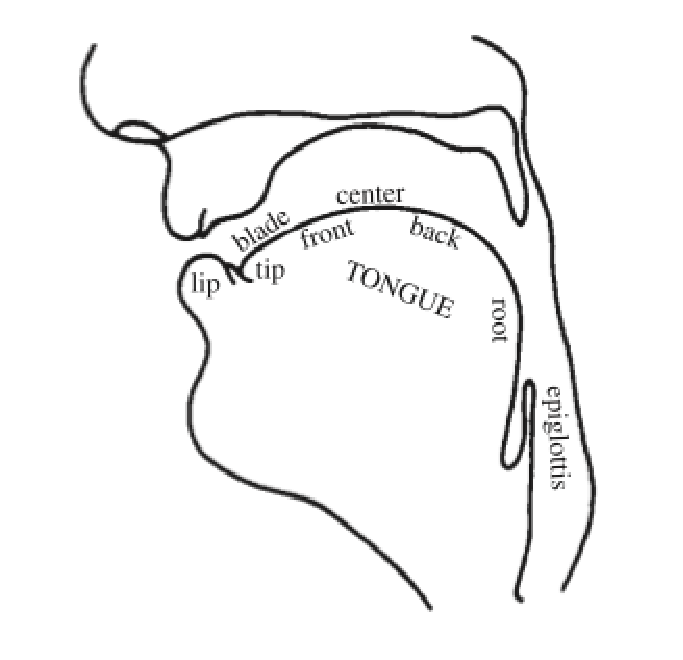
\includegraphics[scale=0.55]{tongue}

\vfill
\columnbreak

\noindent 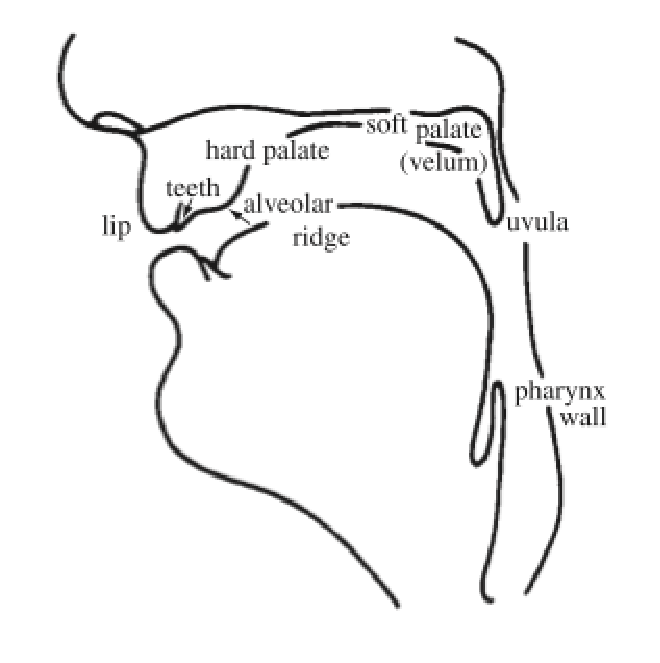
\includegraphics[scale=0.55]{vocaltract}

\end{multicols}

\ex. The vocal folds are held together along their length with enough tension to allow vibration. Table \ref{fig: laryngeal} shows the cycle that they undergo each time you speak --- the so called {\bfseries laryngeal mechanism}:
\a. The vocal folds momentarily block airflow from the lungs
\b. The air pressure underneath the vocal folds increases
\c. The increased pressure forces the vocal folds up and apart 
\d. s the pressure falls again, the vocal folds snap back together 
\e. Go to 1

\begin{figure}[h!]
\caption{The cycle of the laryngeal mechanism}
\label{fig: laryngeal}
\centering
\includegraphics{laryngeal_m.png}
\end{figure}

\ex. Each repetition of cycle in Fig \ref{fig: laryngeal} causes a {\itshape glottal pulse}. The number of times this occurs in a second is the {\itshape fundamental frequency} of voice F$_{0}$, which is one of the primary acoustic correlates of pitch. Varying the tension of the vocal folds results in different rates of vibration, and so different pitches.

\ex. Any sound involving vibration of vocal folds is {\bfseries voiced}; {\bfseries unvoiced sounds} are produced with no vibration of vocal folds.

\ex. {\bfseries Sonorants} are sounds produced with an {\itshape inherent vibration of vocal folds}; therefore, they are {\itshape naturally} voiced.
\a. Glides (aka semiconsonants or approximants): e.g., w, j
\b. Laterals: e.g., l, \textipa{L}
\c. Rhotics: e.g., r, \textipa{R}, \textipa{\;R}
\d. Nasals: e.g., n, m, \textipa{N}, \textltailn, \textipa{M}
\e. {\bfseries Vowels} are sonorant sounds produced with {\itshape \bfseries no obstruction} in the vocal tract. They are described in terms of the movement of the tongue:
	\a. {\itshape body height}: high, mid, low
	\b. {\itshape body advancement}: front, central, back
	\c. {\itshape lip rounding}: rounded or not
	\d. {\itshape root advancement}: tense, lax
	\z.
\f. As opposed to simple vowels (also called {\itshape monophthongs}), {\bfseries diphthongs} are complex vocalic segments made of two vowel sounds, uttered in a single breath.

\begin{figure}[h!]
\centering
\includegraphics{vowels}
\end{figure}

\ex. {\bfseries Consonants} are sounds produced with an {\bfseries obstruction} at any point of the vocal tract. They are described in terms of {\bfseries three aspects}:
\a. The {\bfseries state of the glottis}: are vocal folds vibrating? (see 9-10)
\b. The {\bfseries place of articulation}: {\itshape where} is the restriction?
	\a. Bilabial	
	\b. Labiodental	
	\c. Interdental		
	\d. Alveolar
	\e. Palatal
	\f. Velar
	\f. Glottal
	\z.
\c. The {\bfseries manner of articulation}: {\itshape how} is the restriction produced?
	\a. Stops: {\bfseries complete blockage} of the air due to an active articulator touching a passive one, then a release
	\b. Fricatives: a minimal space between active and passive articulators creates {\bfseries turbulence}
	\c. Affricates: stop+fricative (in this order)

\ex. The properties described above are called {\bfseries segmental}. {\bfseries Suprasegmental properties} concern with larger stretches of speech, such as {\itshape length, stress, tone, intonation.}

\ex. All English sounds and relative IPA symbols are listed below.

\begin{figure}[h!]
\centering
\includegraphics[scale=0.75]{consonants.png}
\end{figure}

\begin{figure}[h!]
\centering
\includegraphics[scale=0.75]{vowels_IPA.png}
\end{figure}

\newpage

\subsection{Activity 3: IPA transcription}

{\itshape Identify the English words correspondent to the following IPA transcriptions. Refer to the tables above.}

\begin{enumerate}
\begin{multicols}{2}
	\parbox{0.3\textwidth}{%
	\item {[}r\textipa{2}bd{]} \hfill \underline{\hspace{1cm}}
	\item {[}r\textscripta mo\textipa{U}s\textschwa s{]} \hfill \underline{\hspace{1cm}}
	\item {[}nid\textschwa d{]} \hfill \underline{\hspace{1cm}}
	\item {[}fi{]} \hfill \underline{\hspace{1cm}}
	\item {[}ne\textipa{IS}n{]} \hfill \underline{\hspace{1cm}}
	\item {[}st\textipa{OpIt}{]} \hfill \underline{\hspace{1cm}}
	\item {[}kr\textipa{O}ld{]} \hfill \underline{\hspace{1cm}}
	\item {[}\textipa{TisIs}{]} \hfill \underline{\hspace{1cm}}
	\item {[}str\textipa{ENT}{]} \hfill \underline{\hspace{1cm}}
	\item {[}stip{]} \hfill \underline{\hspace{1cm}}
	\item {[}gre\textipa{I}s{]} \hfill \underline{\hspace{1cm}}
	\item {[}\textipa{wOrm}{]} \hfill \underline{\hspace{1cm}}
	\item {[}k\ae mr\textipa{@}{]} \hfill \underline{\hspace{1cm}}
	\item {[}h\ae pi{]} \hfill \underline{\hspace{1cm}}
	\item {[}swit{]} \hfill \underline{\hspace{1cm}}
	}	

\columnbreak

	\parbox{0.3\textwidth}{%
	\item {[}pl\ae nd{]} \hfill \underline{\hspace{1cm}}
	\item {[}riz\textipa{2}lt{]} \hfill \underline{\hspace{1cm}}
	\item {[}pr\textepsilon st{]} \hfill \underline{\hspace{1cm}}
	\item {[}bif{]} \hfill \underline{\hspace{1cm}}
	\item {[}e\textipa{IZ@}{]} \hfill \underline{\hspace{1cm}}
	\item {[}\textipa{sINgl}{]} \hfill \underline{\hspace{1cm}}
	\item {[}m\textscripta \textipa{UntIn}{]} \hfill \underline{\hspace{1cm}}
	\item {[}\textipa{TizIs}{]} \hfill \underline{\hspace{1cm}}
	\item {[}\textipa{tIptoU}{]} \hfill \underline{\hspace{1cm}}
	\item {[}st\textepsilon p{]} \hfill \underline{\hspace{1cm}}
	\item {[}gr\ae s{]} \hfill \underline{\hspace{1cm}}
	\item {[}w\textsubdot{r}m{]} \hfill \underline{\hspace{1cm}}
	\item {[}zu{]} \hfill \underline{\hspace{1cm}}
	\item {[}b\textsubdot{r}\textipa{TdeI}{]} \hfill \underline{\hspace{1cm}}
	\item {[}\textipa{lioU}{]}  \hfill \underline{\hspace{1cm}}
	}
\end{multicols}
\end{enumerate}

\newpage

\subsection{Activity 4: Mistaken transcription}

{\itshape Find the errors in the following broadly transcribed words.}

\begin{center}
\begin{tabular}{ l c c c c}
a. & bedroom & [\textipa{bEdrom}] & {\itshape should be} & [\hspace{2cm}] \\
b. & umbrella & [umbr\textepsilon l\textschwa] & {\itshape should be} & [\hspace{2cm}] \\
c. & tea chest & [ti\textteshlig est] & {\itshape should be} & [\hspace{2cm}] \\
d. & visited & [\textipa{vIsIt@d}] & {\itshape should be} & [\hspace{2cm}] \\
e. & football & [\textipa{fUtbol}] & {\itshape should be} & [\hspace{2cm}] \\
f. & bowl & [bol] & {\itshape should be} & [\hspace{2cm}] \\
g. & owl & [\textipa{oUl} & {\itshape should be} & [\hspace{2cm}] \\
h. & shut & [sh\textipa{2}t] & {\itshape should be} & [\hspace{2cm}] \\
i. & theme & [\textipa{D}im] & {\itshape should be} & [\hspace{2cm}] \\
j. & them & [\textipa{D}em] & {\itshape should be} & [\hspace{2cm}] \\
k. & thin & [\textipa{T}in] & {\itshape should be} & [\hspace{2cm}] \\
l. & rang & [r\ae ng] & {\itshape should be} & [\hspace{2cm}] \\
m. & voice & [vois] & {\itshape should be} & [\hspace{2cm}] \\
n. & child & [\textteshlig ild] & {\itshape should be} & [\hspace{2cm}] \\
\end{tabular}
\end{center}

\subsection{Activity 5: Voiced or not?}

{\itshape Is the first sound in each of the following words voiced or voiceless? What about the last sound?}

\begin{center}
\begin{tabular}{ l | p{1cm} | p{1cm} || l | p{1cm} | p{1cm} || l | p{1cm} | p{1cm}}
	& {\itshape First} & {\itshape Last} &		&	{\itshape First} & {\itshape Last} &	& {\itshape First} & {\itshape Last} \\ \hline
a. this & 	&	& e. though &	&	& i. knowledge &		& 	\\ \hline
b. these & 	&	& f. games &	&	& j. pressed &		& 	\\ \hline
c. thin  & 	&	& g. stew &	&	& k. nobody &		& 	\\ \hline
d. thought & 	&	& h. huge &	&	& l. rocks &		& 	\\ \hline
\end{tabular}
\end{center}

\subsection{Activity 6: IPA symbols}

{\itshape Give the phonetic transcription that corresponds to each of the following articulatory descriptions.}

\begin{center}
\begin{tabular}{ l l l }
a.	&	 voiceless velar stop	& [\hspace{2cm}] \\
b.	&	voiceless labiodental fricative & [\hspace{2cm}] \\
c.	&	voiceless palatal affricate	& [\hspace{2cm}] \\
d.	&	voiced interdental fricative	 & [\hspace{2cm}] \\
e.	&	voiced bilabial glide	&	[\hspace{2cm}] \\
f.	&	voiced alveolar fricative	&	[\hspace{2cm}] \\
\end{tabular}
\end{center}

\subsection{Activity 7a: Place and manner of articulation}

{\itshape For each of the following pairs of sounds, state whether they have the same or different place of articulation. Then identify the place of articulation for each sound.}

\begin{center}
\begin{tabular}{ l l l || l | l }
	&		&				&	S/D?		&	Place of articulation? \\ \hline
a.	& 	[s]	&	[\textipa{S}]	&			&					\\
b.	&	[\textipa{N}	&	[g]	&			&					\\
c.	&	[k]			&	[h]	&			&					\\
d.	&	[d]			&	[\textipa{R}]	&			&					\\
e.	&	[w]			&	[m]	&			&					\\
f.	&	[\textipa{Z}]	&	[\textteshlig]	&			&					\\
g.	&	[h]			&	[k]			&			&					\\
h.	&	[l]			&	[z]			&			&					\\
\end{tabular}
\end{center}

\subsection{Activity 7b: Articulation (I)}

{\itshape Circle with words that:}

\begin{center}
\begin{tabular}{ l l l l l l l l }
a. &	begin with a bilabial: & met & net & set & bet & let & pet \\
b. &  begin with a velar:	& knot & got & lot & cot & hot & pot \\
c. &  begin with a labiodental: & fat & cat & that & mat & chat & vat \\
d. & begin with an alveolar: & zip & nip & lip & sip & tip & dip \\
e. & end with a fricative: & race & rose & bush & rave & bring & cough \\
f.  & end with a nasal: & rain & rang & dumb & deaf & sum & lamp \\
g. & end with a stop: & pill & lip & pain & crab & dog & hide \\
\end{tabular}
\end{center}

\newpage

\subsection{Activity 7c: Articulation (II)}

{\itshape Which sounds can correspond to the diagrams below?}

\begin{figure}[h!]
\centering
\includegraphics[scale=0.5]{articulation_ex}
\end{figure}

\subsection{Speech sounds of the world}

\ex. Useful websites:
	\a. \url{http://web.uvic.ca/ling/resources/ipa/charts/IPAlab/IPAlab.htm}
	\b. \url{http://www.uiowa.edu/~acadtech/phonetics/english/frameset.html}
	\c. \url{http://sail.usc.edu/span/rtmri_ipa/index.html}
	\d. \url{http://phonetics.ucla.edu/course/chapter2/amercons.html}
	\e. \url{http://phonetics.ucla.edu/course/chapter2/amerenglishvowels.html}
	\f. \url{http://www.internationalphoneticalphabet.org/ipa-sounds/ipa-chart-with-sounds}
	\f. \url{http://web.uvic.ca/ling/resources/ipa/charts/IPAlab/IPAlab.htm}
	\f. \url{http://www.ipachart.com/}
	\f. \url{http://linguistics.berkeley.edu/acip/course/chapter2/}
	
\ex. Quirky sounds not found in English.
\a. {\itshape Front rounded vowels:}
	\a. [y] like [i] with rounding: German {\" u}
	\b. [ø] like [e] with rounding, German {\" o}
	\c.[{\itshape example:}] \hspace{0.02cm} ger. schon [\textipa{S}on{] }`already'; sch{\" o}n [\textipa{S}øn] `beautiful'
	\z.
\b. {\itshape Nasalized vowels:} vowels produced with the velum lowered. Nasalized is indicated with a tilde `$\sim$' over the vowel: e.g., [{\~e}].
	\a.[{\itshape example:}] \hspace{0.02cm} fr. chasse [\textipa{S}\textscripta s{]} `hunt'; chance [\textipa{S}{\~ \textscripta}s{]} `luck'
	\z.
\c. {\itshape special fricatives:}
	\a. bilabial fricatives: voiceless [\textipa{F}], voiced [\textipa{B}] ({\' E}w{\' e}, a Niger-Congo language spoken by 2.5m people in Ghana)
	\b. velar fricatives: voiceless [x], voiced [\textipa{G}] (Modern Greek)
	\z.
\d. {\itshape Palatals}:
	\a. Voiceless post-palatal [c]
	\b. nasal palatal [\textltailn]
	\c. voiceless fricative [ç]
	\z.
\e. {\itshape Uvulars}: produced with the uvula, the fleshy tab hanging from the velum. For example, Farsi has:
	\a. Voiceless stop [q]
	\b. voiced stop [\textipa{\;G}]
	\z.
\f. {\itshape Pharyngeals}: produced with pharynx, the lower section of throat just above the larynx.
	\a. Voiceless fricative [\textcrh]
	\b. voiced fricative [\textrevglotstop] (Hebrew)
	\z.
\f. {\itshape Secondary manner of articulation}
	\a. palatalization: e.g., [n$^{j}$]
	\b. glottalization: closure of glottis simultaneous with oral stop, [p\textsuperscript{\textglotstop}]
	\c. velarization: e.g. `dark l' in English -- [\textltilde] as in `all'
	\z. 
\f. The most common airstream mechanism is called {\itshape pulmonic egressive}, where the air is pushed out of the lungs by the ribs and diaphragm. There is also a glottalic airstream mechanism, which initiates airflow in the upper vocal tract by means of the glottalic area (i.e., the vocal cords). If the larynx raises, {\itshape ejective consonants} are produced; when the closure of the glottis. If the larynx lowers, {\itshape implosive consonants} are produced instead.

\newpage

\section{Acoustic phonetics}

\ex. Certain vibrating bodies --- like tuning forks --- produce a pure periodic sinusoidal (sine-like) sound wave.	

\begin{figure}[h!]
\centering
\includegraphics{waves}
\end{figure}

\ex. The sounds produced can be classified by a number of physical properties.  The two we are most interested in are {\itshape amplitude} (how high the wave is) and {\itshape frequency} (measured in Hz, cycles per second). In terms of sound perception, amplitude corresponds roughly to {\itshape loudness}, and frequency corresponds roughly to {\itshape pitch}.

\ex. The vocal folds (and tract) are not tuning forks, they cannot vibrate in such a simple way. The vocal folds instead produce a complex wave.  For example:

\begin{figure}[h!]
\centering
\includegraphics{forks}
\end{figure}

\ex. Although this wave is complex, it is still possible to discern an over cycle of repetition.  The number of these per second is the fundamental frequency (F$_{0}$) of the sound wave. We know from math (Fourier analysis) that every periodic wave can be analyzed into the composition of simpler sine waves. Natural media like strings and vocal folds vibrate not only at their fundamental frequency but at every integer multiple of F$_{0}$ as well.  These higher frequencies are the harmonics of the fundamental frequency.  The higher the harmonic, the lower the amplitude.  Here is what the harmonics of a 100Hz F$_{0}$ look like.

\begin{figure}[h!]
\centering
\includegraphics{amplitude}
\end{figure}

\ex. The graph above is called a {\itshape spectrum}; it represents the amplitude of sound waves at a variety of frequencies at one point in time.

\ex. The rest of the vocal tract acts as a {\itshape filter} on the complex wave produced by the vocal folds.  The natural {\itshape resonances} of the vocal cavity will amplify certain frequencies and dampen others.  Here is what the spectrum of a typical vowel sound looks like:

\begin{figure}[h!]
\centering
\includegraphics{resonances}
\end{figure}

\ex.[] Notice that after filtering the spectrum no longer has an even distribution of energy; there are distinct peaks.  These peaks are called the {\itshape formants} of the speech sound.  

\ex. It is important to understand that the natural resonances of the vocal tract change as it assumes different configurations.  Thus, each vowel has a distinct formant structure.  A typical way to represent the physical properties of a vowel or speech sound is a 3-D spectrogram. A spectrogram represents the spectrum over time. Frequency is plotted against time.  The third dimension, amplitude, is represented by degree of darkness at a point.

\begin{figure}[h!]
\centering
\includegraphics[scale=0.5]{formants}
\caption{Spectrogram of [\ae], generated with PRAAT}
\end{figure}

\ex. There are some simple generalizations that are worth knowing:
\a. F1 and tongue height are inversely correlated: the higher F1 is the lower the height of the vowel.
\b. F2 and tongue fronting are correlated: the higher F2 is the farther forward the tongue is in the mouth.

\section{Recap}

\ex. Phonetics is the science of sounds humans can produce with their vocal tract, from a purely articulatory point of view. 

\ex. Writing systems may sometimes be opaque in representing sounds. The International Phonetic Alphabet is a internationally accepted set of symbols, each of which corresponds to exactly one sound.

\ex. Sounds are produced by the rhythmic opening and closure of the vocal folds, muscular membranes right above the epiglottis and the trachea. When vocal folds vibrate, they produce a voiced sound; when they do not vibrate, they produce an unvoiced sound.

\ex. Sonorants are sounds that are inherently voiced (i.e., they always involve vibration of vocal folds). Vowels are sonorant sounds involving no obstruction in the vocal tract.

\ex. Consonants involve some degree of obstruction in the vocal tract. They are described in terms of vocal fold vibration (i.e., voiced/unvoiced), place of articulation (where the obstruction occurs) and manner of articulation (the degree of obstruction).

\ex. Suprasegmental properties concern higher portions of speech: e.g., length, stress, tone, intonation.

\ex. All languages have pulmonic egressive sounds, which are produced by pushing the air out of the lungs by the ribs and diaphragm. Some languages also have ejective and implosive sounds, which are produced by pushing the air out of the lungs with the help of the glottis.

\ex. As they are, sounds are auditory waves. Linguists are mostly interested in formants, concentration of acoustic energy around a particular frequency in the speech wave. This is because formant values apparently correlate with different configurations of the tongue in the vocal tract.


\end{document}